\subsection{Quantitative data}

    %What the data said

    \subsubsection{Big formative app test}
  The app test simulated the app being used to assess preparedness for a youth session. The test clearly showed evidence between the difference between designing for Assessment and Learning. See figure \ref{fig:summativeTest} and figure \ref{fig:computerTest} to understand the setting.

  Before the quiz started, the coaches were asked to raise their hand if they felt proficient with using a smart phone. 8 out of 23 said yes. After using the app, 16 thought they were proficient (25\% increase), while 5 said low proficiency, and 2 said no (we don't yet feel proficient, still fear).

  The test was done in pairs, because of lack of devices.

  \begin{figure}[h]
    \centering
    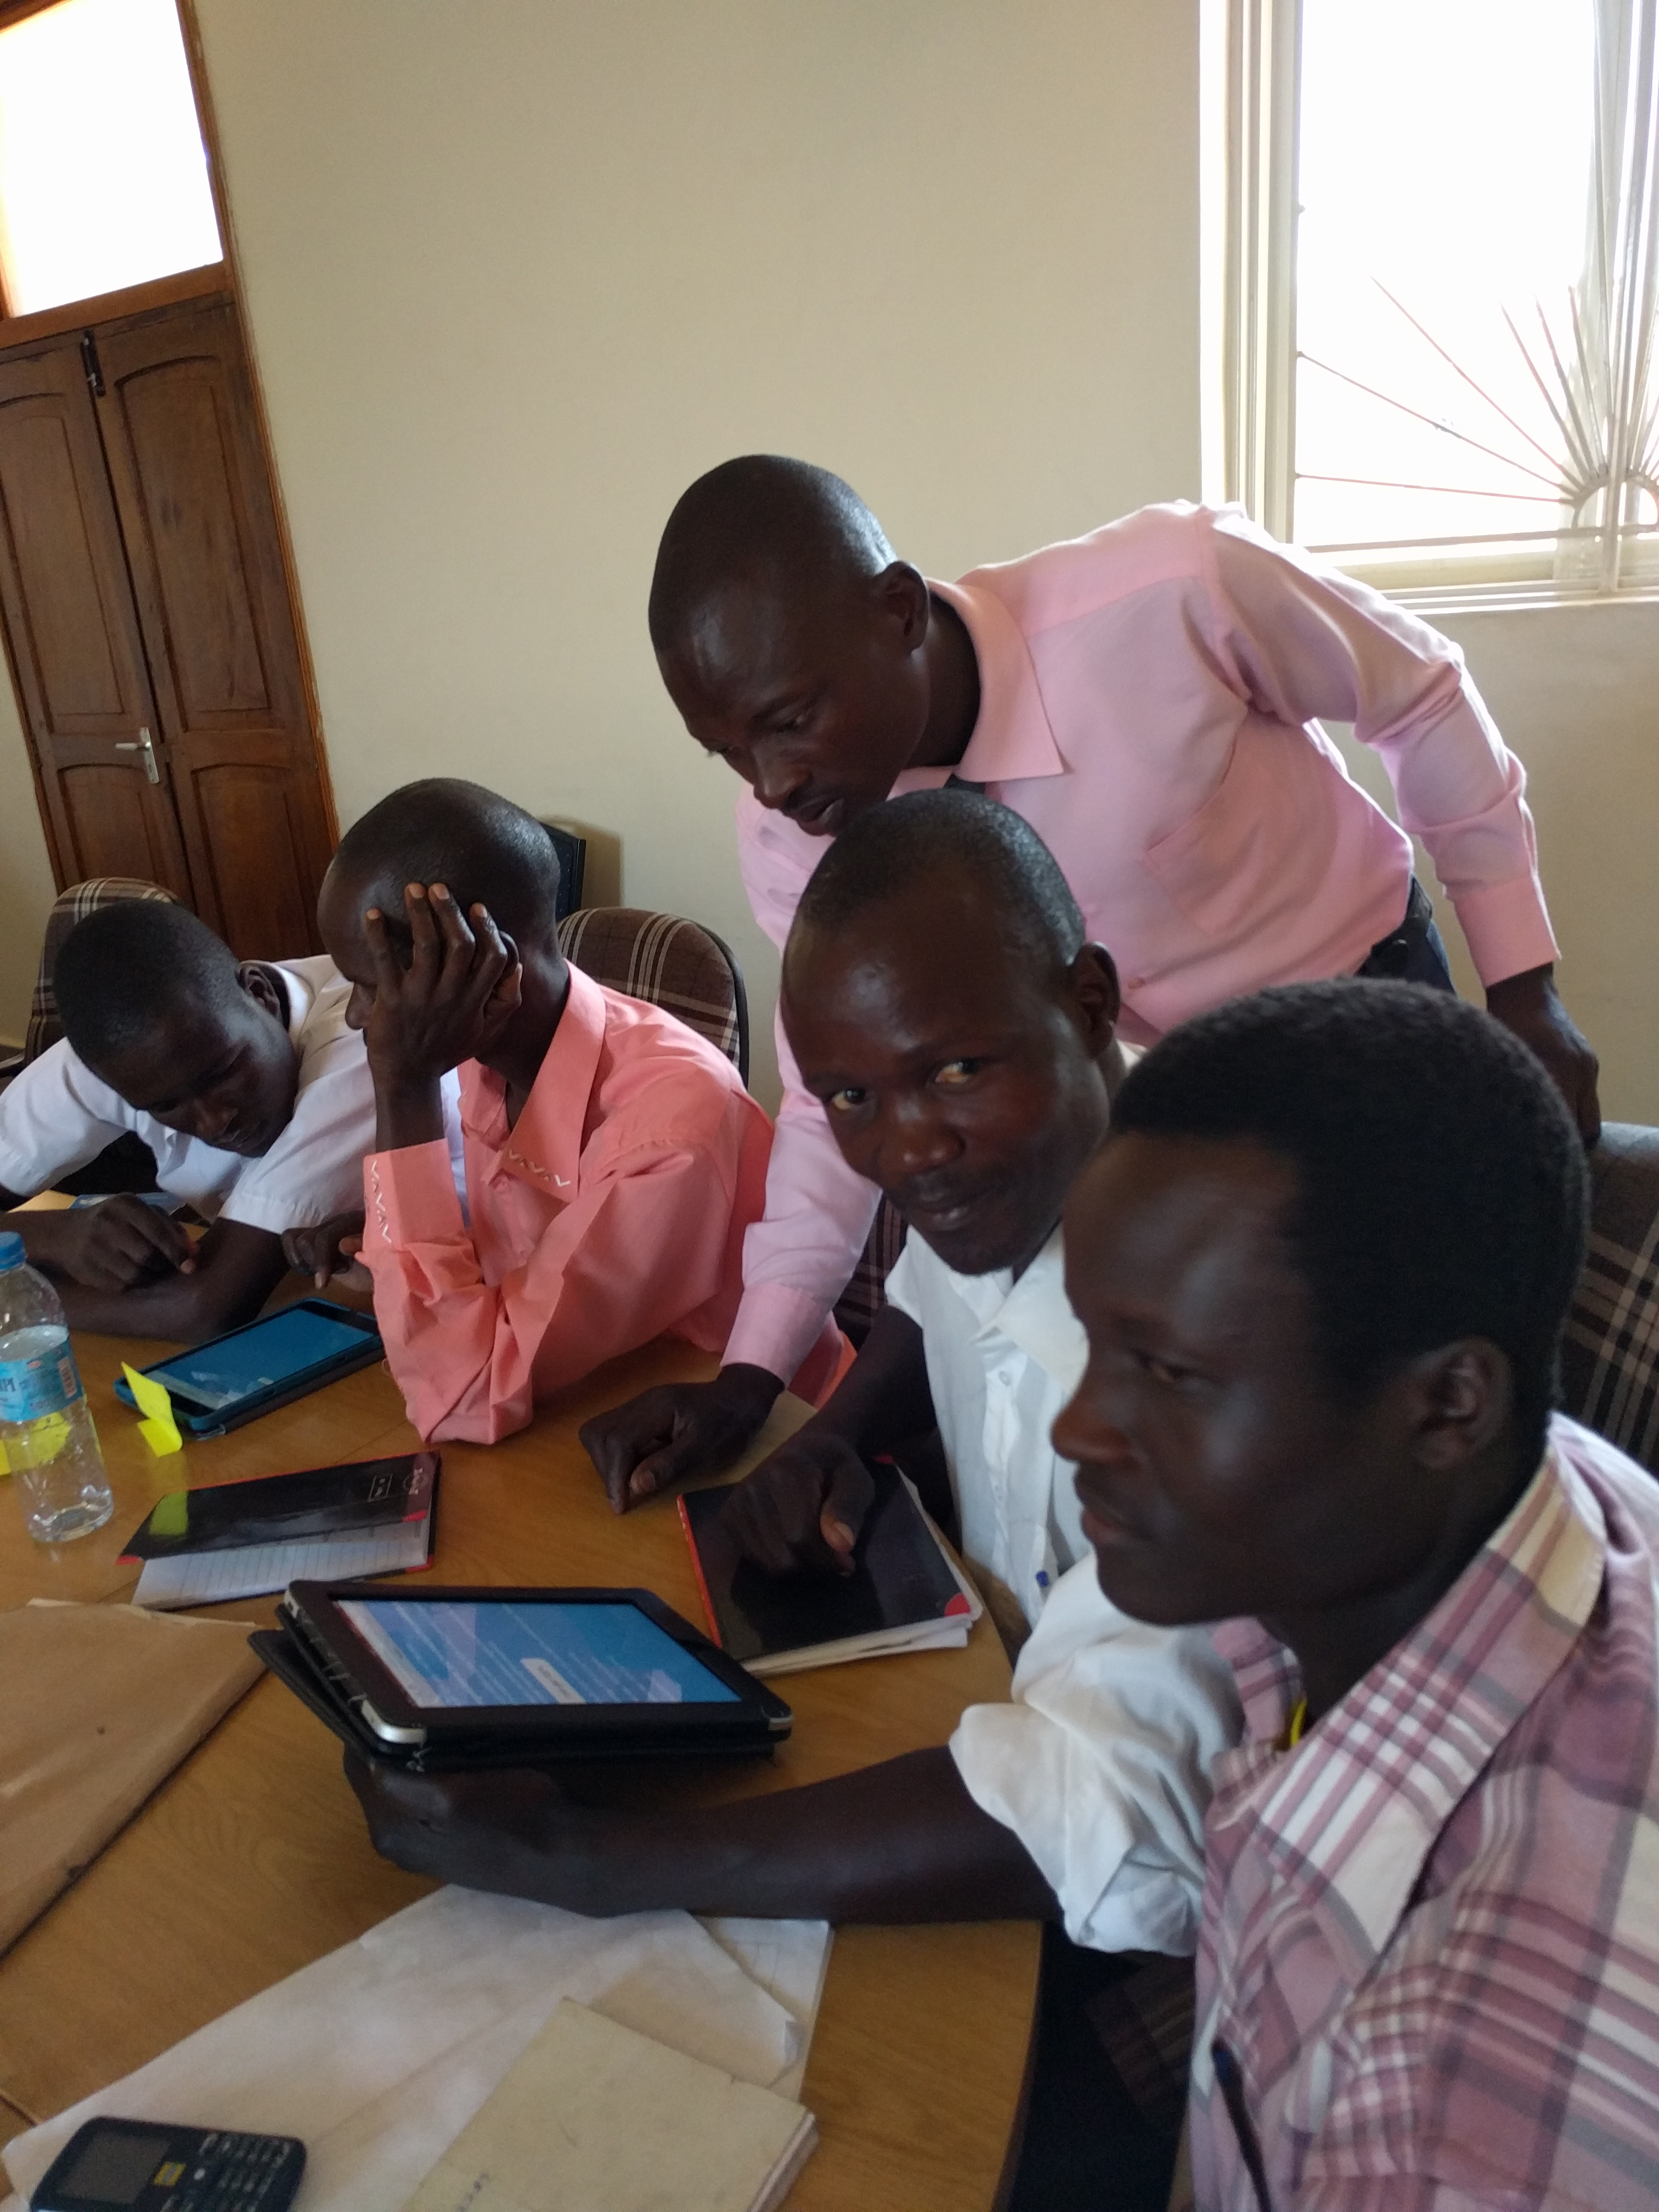
\includegraphics[width=0.8\textwidth]{appTestTablet.png}
    \caption{Two coaches using a tablet for the formative app test. The coaches worked in pairs. After the app test, interviews was held, before co-creation workshops started.}
    \label{fig:tabletTest}
  \end{figure}

  \begin{figure}[h]
    \centering
    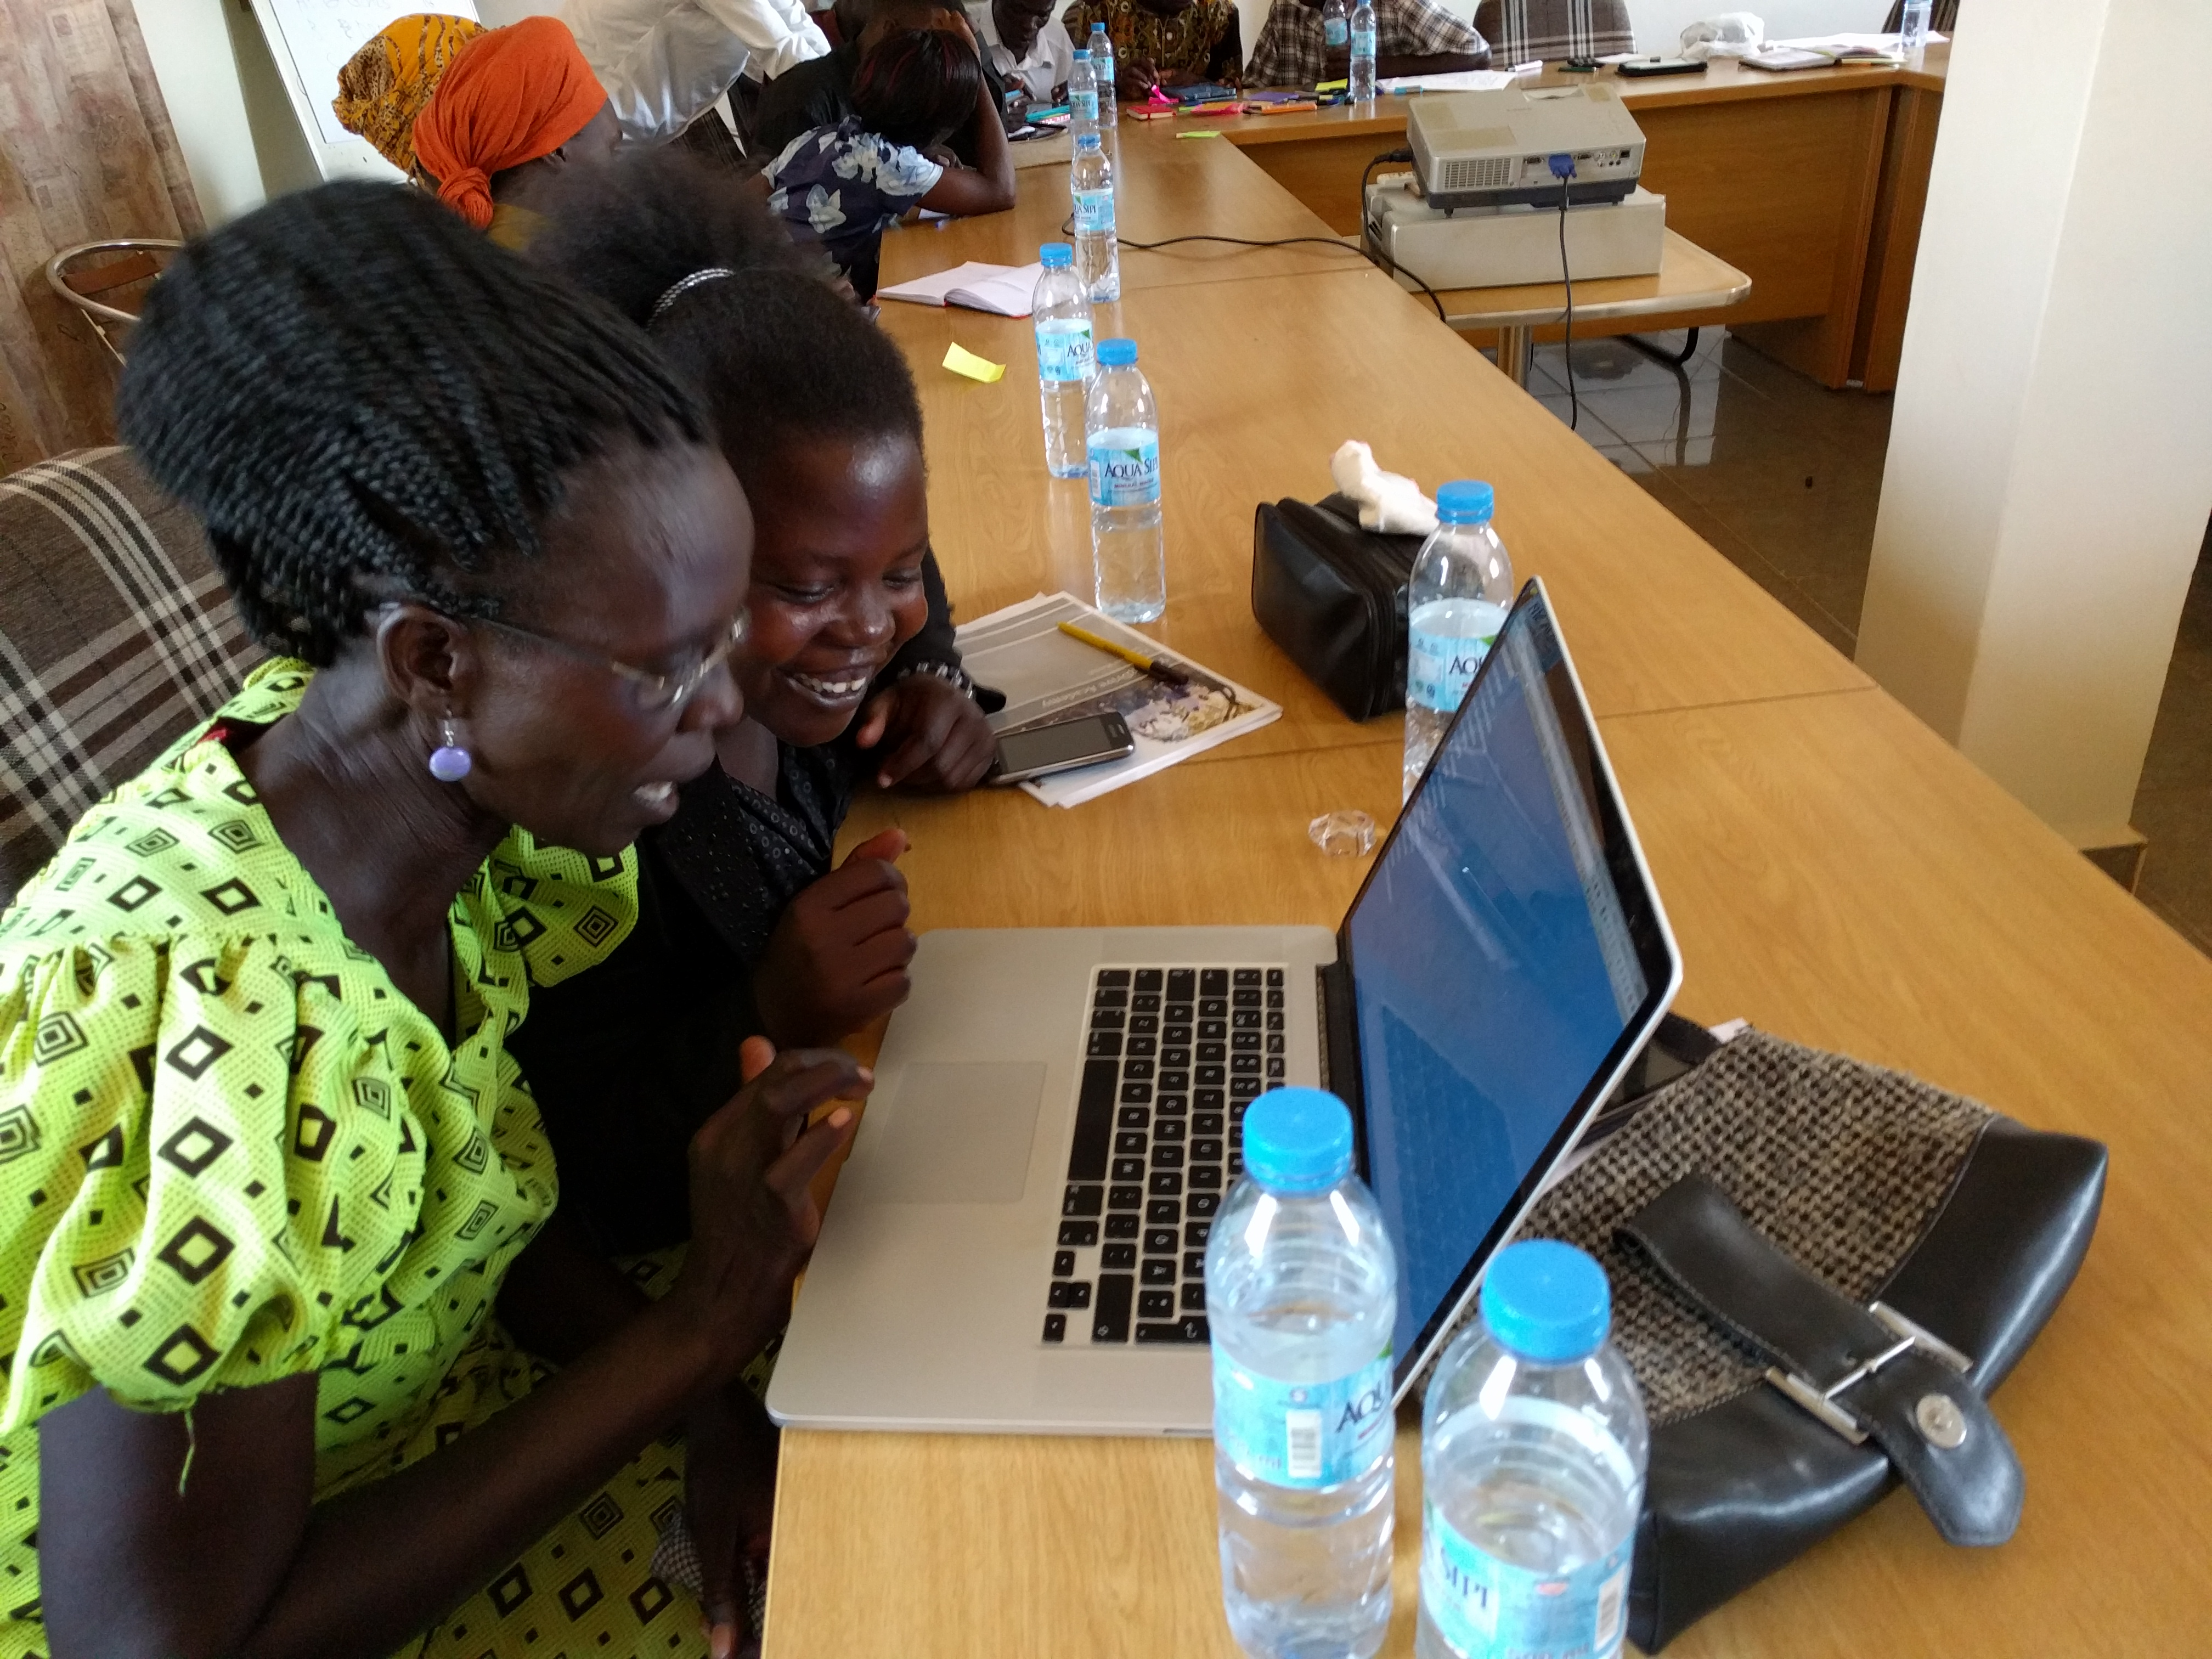
\includegraphics[width=0.8\textwidth]{appTestComputer.png}
    \caption{A variation of smartphones and tablets were used. In one case, the battery died on one of the device so it needed to be replaced with a computer. It was the first time the coaches used a computer, and they learned quickly and eagerly.}
    \label{fig:computerTest}
  \end{figure}

  Regarding usability, the most negative thing from the app test, was that the app was not user friendly for 1st-time smartphone users. There were a lot of bugs, the most damaging for the app test being resizing of the font size for each new question, see figure \ref{fig:iteration-map} E-3. This forced some coaches to try to zoom on the devices, even if they did not know how. This could in turn cause refresh of the web page, and sometimes there was no Internet available. Thus, the data can not be fully reliable.

  This was the first time true frustration was shown. Out of 23 respondents, 7 rated the app easy, 11 medium, and 6 hard. This was not viable.

  Regarding learning, cognitive load seemed to be too high. The feedback was not scaffolded enough, so coaches did not have enough energy to assess all of their results carefully before taking the test again via "Improve". One user did not want to press "Improve" until having read the manual. The motivation was: "Not because that is what the info says, but because I can learn more from the manual, about more than what the questions says." This is in fact the preferred behaviour from Josefina, and the app should continue to further encourage only using the app training or certification mode after having prepared via the manual. This way, the app is still assessment, but it is "learning by thinking", with feedback. In iteration 4, comparing those that are allowed to use the manuals with those that are not allowed to, would be interesting.
